\section{MMSE and MAP estimators}

\subsection{a}

\begin{figure}[H]
 \centering
 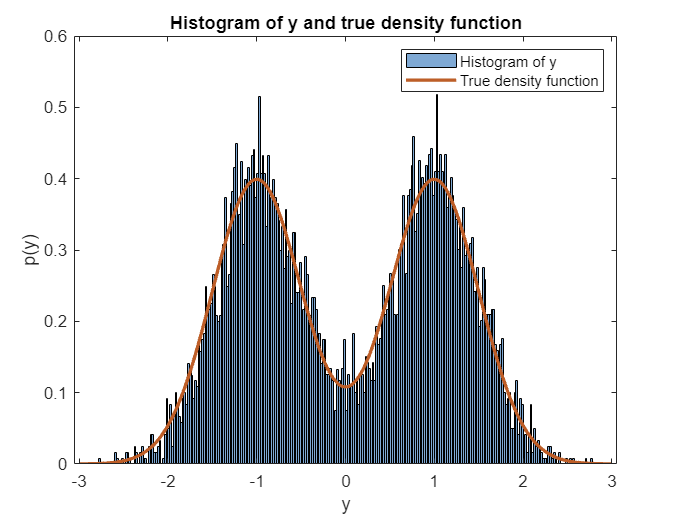
\includegraphics[width=0.7\textwidth]{images/graphfor4a.png}
 \caption{Sample 3000 times }
 \label{4a}
\end{figure}

Since $\theta$ is equally likely to be -1 or 1, the histogram of y should show two normal distributions with means -1 and 1 and equal variances $\sigma^2 = 0.25$. The overall shape of the histogram should be a bimodal distribution, with two peaks at -1 and 1 and equal weights. This bimodal distribution represents a mixture of two normal distributions, each with a different mean and the same variance.

\subsection{b}

\emph{Note: In my homework, solving b is after c. So I used the conclusions in c to prove b while.}

In this problem, we are given that $y = \theta + w$, where $w \sim N(0, 0.25)$ is a normally distributed noise term with mean 0 and variance 0.25. Therefore, the probability density function of y given theta is given by:

$$p(y | \theta) = \frac{1}{\sqrt{2\pi\sigma^2}} \exp \left(-\frac{(y - \theta)^2}{2\sigma^2}\right)$$

From c, we get:

$$p(y) = 0.5 \cdot \frac{1}{\sqrt{2 \pi \sigma^2}} \exp \left(-\frac{(y - 1)^2}{2 \sigma^2}\right) + 0.5 \cdot \frac{1}{\sqrt{2 \pi \sigma^2}} \exp \left(-\frac{(y + 1)^2}{2 \sigma^2}\right)$$

Substituting $y=0.7$ and $sigma^2$ = 0.25, we obtain:
\begin{lstlisting}
q = @(theta,y) 1/sqrt(2*pi*sigma2)*exp(-(y-theta)^2/(2*sigma2));
q(1,0.7)
ans =

    0.6664


f = @(y) 0.5*1/sqrt(2*pi*sigma2)*exp(-(y-1)^2/(2*sigma2))+0.5*1/sqrt(2*pi*sigma2)*exp(-(y+1)^2/(2*sigma2));
f(0.7)

ans =

    0.3345
\end{lstlisting}

so:

$p(\theta=1 | y=0.7) = \frac{p(y=0.7 | \theta=1) p(\theta=1)}{p(y=0.7)} = \frac{0.6664\times0.5}{0.3345}=0.9961$

$$p(\theta=-1 | y=0.7) = 0.0039$$

So I guess $ \theta $ =1.

\subsection{c}

To prove that $p(y)$ is a mixture of two normal distributions with means $-1$ and $1$ and the same variance $\sigma^2$, we can use the law of total probability.

In this problem, we can partition the sample space of $y$ into two mutually exclusive events: $y = \theta + w$ where $\theta = 1$ and $\theta = -1$, where $w \sim \mathcal{N}(0, \sigma^2)$ is a normally distributed noise term with mean $0$ and variance $\sigma^2$. 

Using the law of total probability, we can express $p(y)$ as a mixture of the two normal distributions as follows:

$$p(y) = p(y | \theta = 1) p(\theta = 1) + p(y | \theta = -1) p(\theta = -1)$$

where $p(y | \theta = 1)$ is the probability density function of the normal distribution with mean $1$ and variance $\sigma^2$, and $p(y | \theta = -1)$ is the probability density function of the normal distribution with mean $-1$ and variance $\sigma^2$.

Substituting the expressions for the two probability density functions, we obtain:

$$p(y) = 0.5 \cdot \frac{1}{\sqrt{2 \pi \sigma^2}} \exp \left(-\frac{(y - 1)^2}{2 \sigma^2}\right) + 0.5 \cdot \frac{1}{\sqrt{2 \pi \sigma^2}} \exp \left(-\frac{(y + 1)^2}{2 \sigma^2}\right)$$

Therefore, $p(y)$ is a mixture of two normal distributions with means $-1$ and $1$ and the same variance $\sigma^2$.

\subsection{d}

The Bayesian rule says:
\begin{equation}
    \begin{aligned}
        p(\theta|y)= \frac{p(y|\theta)}{p(y)}\nonumber
    \end{aligned}
\end{equation}

Already known $ p(y) $ in question c and $ p(y|\theta) $ in question b, so:

\begin{equation}
    \begin{aligned}
        p(\theta|y)&=\begin{cases}\frac{\frac{1}{2}\frac{1}{\sqrt{2\pi}\sigma}\exp\{-\frac{1}{2\sigma^2}(y-1)^2\}}{\frac{1}{2}\frac{1}{\sqrt{2\pi}\sigma}\exp\{-\frac{1}{2\sigma^2}(y-1)^2\}+\frac{1}{2}\frac{1}{\sqrt{2\pi}\sigma}\exp\{-\frac{1}{2\sigma^2}(y+1)^2\}}& \text{if } \theta =1\\ \frac{\frac{1}{2}\frac{1}{\sqrt{2\pi}\sigma}\exp\{-\frac{1}{2\sigma^2}(y+1)^2\}}{\frac{1}{\sqrt{2\pi}\sigma}\exp\{-\frac{1}{2\sigma^2}(y-1)^2\}+\frac{1}{2}\frac{1}{\sqrt{2\pi}\sigma}\exp\{-\frac{1}{2\sigma^2}(y+1)^2\}}&\text{if } \theta=-1\end{cases}\\
        &=\begin{cases}\frac{\exp\{\frac{y}{\sigma^2}\}}{\exp\{\frac{y}{\sigma^2}\}+\exp\{-\frac{y}{\sigma^2}\}}&\text{if } \theta =1\\ \frac{\exp\{\frac{-y}{\sigma^2}\}}{\exp\{\frac{y}{\sigma^2}\}+\exp\{-\frac{y}{\sigma^2}\}}&\text{if } \theta =-1\end{cases}\\
        &\text{where  }  \sigma^2=0.25\nonumber
    \end{aligned} 
\end{equation}

\subsection{e}

\begin{equation}
    \begin{aligned}
        \:\hat{\theta}_{M M S E}&=\sum_{\theta}\theta\operatorname*{Pr}\{\theta|y\}.\:\\
        &=p(\theta=1|y)-p(\theta=-1|y)\\
        &=\dfrac{\exp\frac{y}{\sigma^2}-\exp-\frac{y}{\sigma^2}}{\exp\frac{y}{\sigma^2}+\exp-\frac{y}{\sigma^2}}\\
        &=\:\:\frac{2\sinh\left(\frac{y}{\sigma^2}\right)}{2\cosh\left(\frac{y}{\sigma^2}\right)}=\tanh\left(\frac{y}{\sigma^2}\right)=tanh(4y)\nonumber
    \end{aligned}
\end{equation}

\subsection{f}

\begin{equation}
    \begin{aligned}
        \hat{\theta}_{MAP}&=\arg\max\limits_{\theta=\pm1}\pi_y(\theta)\nonumber\\
        &=\begin{cases}1& \text{if } \frac{\exp\frac{y}{\sigma^2}}{\exp\frac{y}{\sigma^2}+\exp-\frac{y}{\sigma^2}}\geq\frac{\exp-\frac{y}{\sigma^2}}{\exp\frac{y}{\sigma^2}+\exp-\frac{y}{\sigma^2}}\\-1& \text{if } \frac{{\exp}\frac{y}{\sigma^2}}{\exp\frac{y}{\sigma^2}+\exp-\frac{y}{\sigma^2}}<\frac{{\exp}-\frac{y}{\sigma^2}}{\exp\frac{y}{\sigma^2}+\exp-\frac{y}{\sigma^2}}\end{cases}\\
        &=\begin{cases}1& \text{if } y\geq 0\\-1 & \text{if } y \leq 0 \end{cases}
    \end{aligned}
\end{equation}

\subsection{g}
\subsubsection{1}

In 4b), we made the guess that $\theta$ is 1. Meanwhile, for the specific value of $y=0.7$, both the MMSE estimator and the MAP estimator would predict that $\theta$ is 1. In this case, our guess in 4b coincides with both the MMSE and MAP estimators.

\subsubsection{2}

In this problem, the MMSE and MAP estimators for $\theta$ are different. The MMSE estimator is given by $\hat{\theta}_{MMSE} = \tanh(4y)$, while the MAP estimator is given by $\hat{\theta}_{MAP} = \operatorname{sgn}(y)$.

The MMSE estimator minimizes the expected squared error between the estimated value of $\theta$ and the true value, while the MAP estimator maximizes the posterior probability of $\theta$ given the observation $y$. In this case, the MMSE estimator and the MAP estimator make different decisions when $y$ is close to 0.

If $y$ is positive, both the MMSE and MAP estimators predict that $\theta$ is 1. If $y$ is negative, the MMSE estimator predicts that $\theta$ is -1, while the MAP estimator predicts that $\theta$ is 1. This is because the MMSE estimator takes into account the entire posterior distribution of $\theta$, while the MAP estimator only considers the most probable value of $\theta$.

